% VYSOKOŠKOLSKÁ SEMESTRÁLNÍ PRÁCE
% autor: Lukáš Milar, Tomáš Prudký
% název: Zpracování dat pro předmět NMAST
% !TEX encoding = UTF-8 Unicode
\documentclass[a4paper]{ article}

\usepackage{cmap}
\usepackage[utf8]{inputenc}
\usepackage[T1]{fontenc}
\usepackage[czech]{babel}
\selectlanguage{czech}
\usepackage{vskpupa}

%%%%%%%%%%%%%%%%%%%%%%%%%%%%%%%%%%%%%%%%%%%%%%%%%%%%%%%%%%%%
% Údaje o práci
%%%%%%%%%%%%%%%%%%%%%%%%%%%%%%%%%%%%%%%%%%%%%%%%%%%%%%%%%%%%

\def\jmenoFakulty{Fakulta elektrotechniky a informatiky}
\def\jmenoAutora{Bc. Lukáš Milar, Bc. Tomáš Prudký}
\def\nazevPrace{Zpracování dat pro předmět NMAST}
\def\typPrace{Semestrální práce}
\def\rok{2021}

%%%%%%%%%%%%%%%%%%%%%%%%%%%%%%%%%%%%%%%%%%%%%%%%%%%%%%%%%%%%
% Začátek dokumentu
%%%%%%%%%%%%%%%%%%%%%%%%%%%%%%%%%%%%%%%%%%%%%%%%%%%%%%%%%%%%

\usepackage{Sweave}
\begin{document}
\Sconcordance{concordance:semestralni_prace.tex:semestralni_prace.Rnw:%
1 28 1 1 0 20 1 1 17 6 1 1 11 19 1 1 7 6 1 1 130 20 0 1 7 20 0 1 7 20 0 %
1 2 14 1 1 5 2 1 1 5 13 1 1 5 2 1 1 5 12 1 1 5 2 1 1 5 13 1 1 5 2 1 1 5 %
11 1 1 10 2 1 1 10 12 1 1 10 2 1 1 11 6 1 1 20 2 1 1 20 8 1 1 5 2 1 1 5 %
6 1 1 5 2 1 1 5 6 1 1 5 2 1 1 5 6 1 1 5 2 1 1 5 6 1 1 5 2 1 1 5 7 1 1 5 %
2 1 1 5 6 1 1 5 7 1 1 5 2 1 1 5 5 1 1 5 2 1 1 5 5 1 1 5 8 1 1 7 10 1 1 %
23 20 0 1 2 12 1 1 5 10 1 1 5 8 1 1 8 3 1 1 2 13 0 2 2 13 0 2 2 13 0 1 %
2 2 1 1 2 13 0 2 2 13 0 2 2 13 0 1 2 3 1 1 2 13 0 1 2 6 1 1 2 13 0 2 2 %
13 0 2 2 13 0 1 2 2 1 1 2 13 0 2 2 13 0 1 2 2 1 1 2 8 0 2 2 8 0 1 2 4 1 %
1 2 13 0 1 2 2 1 1 2 7 0 2 2 7 0 1 2 3 1 1 3 10 0 1 2 3 1 1 5 7 1 1 5 2 %
1 1 5 7 1 1 5 2 1 1 5 7 1 1 5 7 1 1 3 5 0 1 2 5 1 1 6 127 0 1 1 43 0 1 %
2 52 0 1 2 4 1 1 5 8 1 1 5 44 0 1 1 1 2 4 1 1 5 2 1 1 5 5 1 1 5 8 1 1 2 %
7 0 1 2 5 1 1 10 7 1 1 16 58 1}


%%%%%%%%%%%%%%%%%%%%%%%%%%%%%%%%%%%%%%%%%%%%%%%%%%%%%%%%%%%%
% Úvodní strany
%%%%%%%%%%%%%%%%%%%%%%%%%%%%%%%%%%%%%%%%%%%%%%%%%%%%%%%%%%%%

\titulniStrana
\generujObsah			% obsah
\generujSeznamObrazku		% seznam obrázků
\generujSeznamTabulek		% seznam tabulek

%%%%%%%%%%%%%%%%%%%%%%%%%%%%%%%%%%%%%%%%%%%%%%%%%%%%%%%%%%%%
% Úvod
%%%%%%%%%%%%%%%%%%%%%%%%%%%%%%%%%%%%%%%%%%%%%%%%%%%%%%%%%%%%


\clearpage
\pagestyle{plain}		% zapne číslování stránek (sazba zápatí)
\phantomsection \addcontentsline{toc}{section}{Úvod}
\section*{Úvod}
\label{uvod}

%% Načítání dat start


%% Načítání dat end

%%%%%%%%%%%%%%%%%%%%%%%%%%%%%%%%%%%%%%%%%%%%%%%%%%%%%%%%%%%%
% Kapitoly
%%%%%%%%%%%%%%%%%%%%%%%%%%%%%%%%%%%%%%%%%%%%%%%%%%%%%%%%%%%%

%% Popis dat
\section{Popis dat}

%% Popisná statistika
\section{Popisná statistika}
% latex table generated in R 4.1.1 by xtable 1.8-4 package
% Thu Nov 18 17:37:30 2021
\begin{table}[ht]
\centering
\begin{tabular}{rrrrrrrrrrr}
  \hline
 & USD & GBP & CHF & EUR & BRL & ILS & CAD & MXN & BGN & RON \\ 
  \hline
prumer & 23.29 & 29.60 & 24.87 & 26.64 & 4.34 & 6.76 & 17.26 & 1.04 & 13.62 & 5.50 \\ 
  modus & 23.59 & 29.36 & 24.28 & 26.68 & 4.40 & 6.81 & 17.13 & 1.01 & 13.81 & 5.51 \\ 
  median & 23.39 & 29.47 & 24.80 & 26.64 & 4.37 & 6.78 & 17.29 & 1.04 & 13.62 & 5.50 \\ 
  max & 25.55 & 31.40 & 26.24 & 27.61 & 4.84 & 7.25 & 18.23 & 1.11 & 14.11 & 5.71 \\ 
  min & 21.88 & 28.69 & 24.13 & 26.06 & 3.92 & 6.43 & 16.46 & 0.98 & 13.32 & 5.38 \\ 
  skewness & 0.51 & 1.07 & 0.84 & 0.64 & 0.02 & 0.41 & 0.18 & 0.03 & 0.64 & 0.79 \\ 
  kurtosis & -0.82 & 0.40 & -0.02 & -0.13 & -0.37 & -0.89 & -0.90 & -0.82 & -0.14 & 0.08 \\ 
  deviation & 1.05 & 0.65 & 0.55 & 0.40 & 0.20 & 0.22 & 0.44 & 0.03 & 0.20 & 0.08 \\ 
  interquartile & 1.48 & 0.71 & 0.68 & 0.52 & 0.26 & 0.32 & 0.68 & 0.05 & 0.27 & 0.10 \\ 
   \hline
\end{tabular}
\caption{Části popisné statistiky aplikované na data} 
\label{table:popisStat}
\end{table}\clearpage

%% Základní grafy
\section{Základní grafy}
\subsection{Histogram}
\begin{figure}[H]
\centering
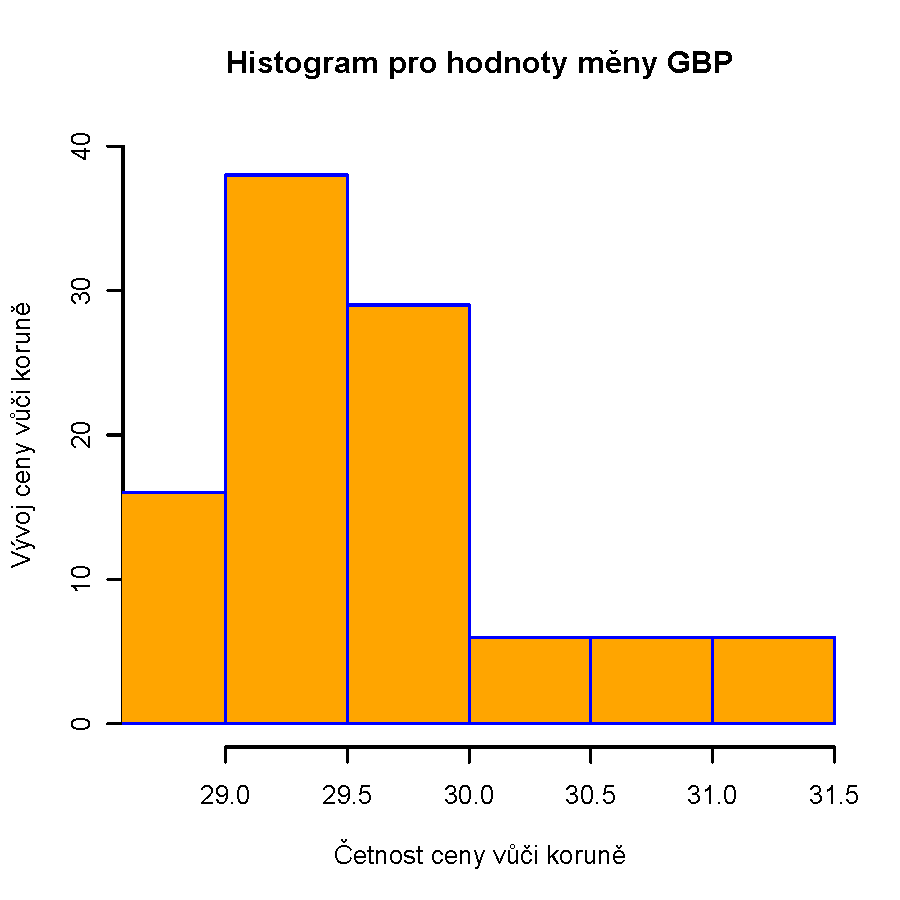
\includegraphics[width=10cm]{histogram_max.pdf}
\caption{Histogram měny s maximální hodnotou šikmosti}
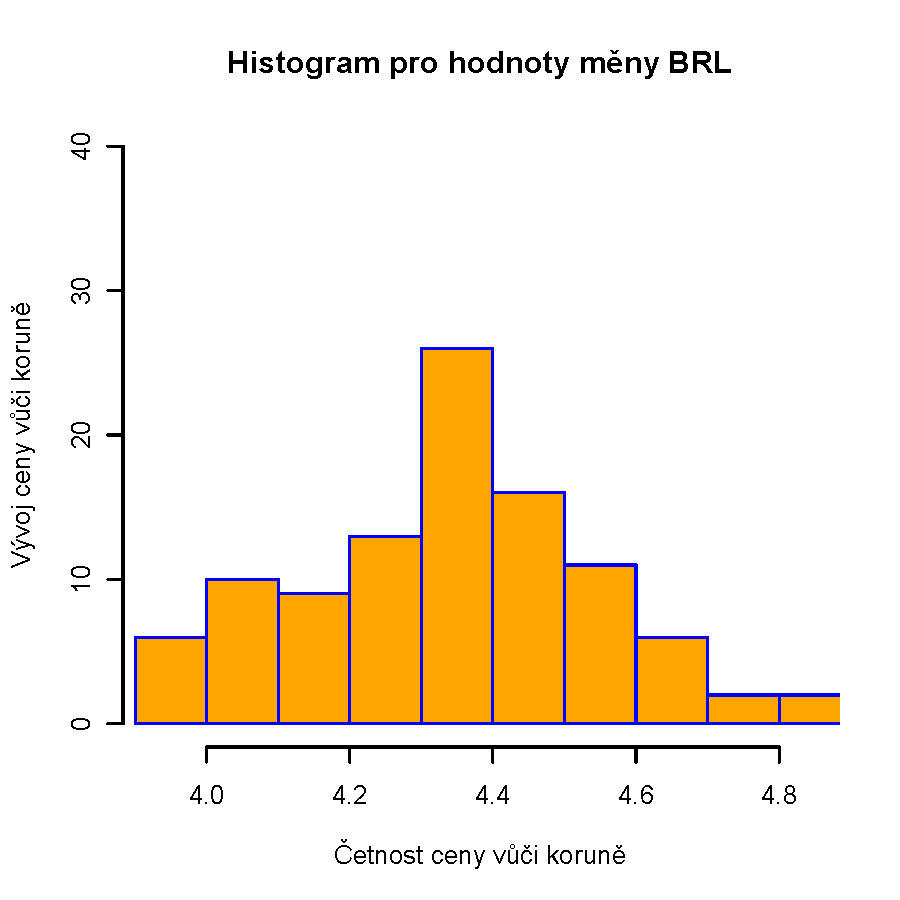
\includegraphics[width=10cm]{histogram_min.pdf}
\caption{Histogram měny s minimální hodnotou šikmosti}
\end{figure}
\subsection{Boxplot}
\begin{figure}[H]
\centering
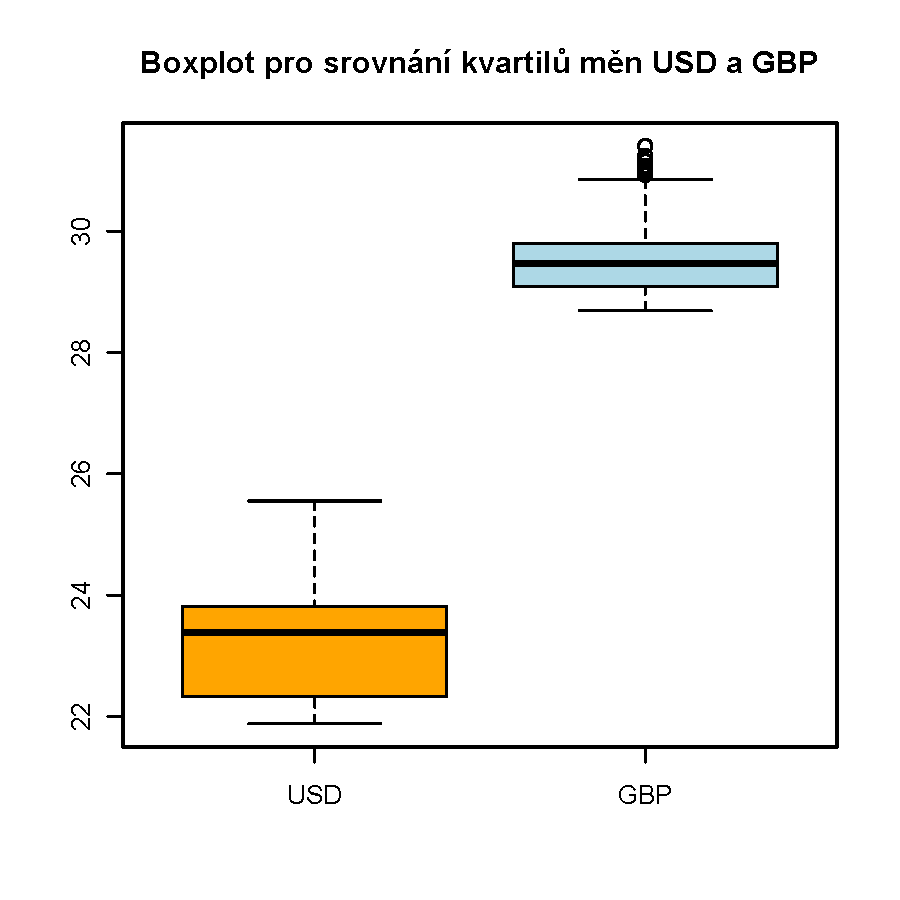
\includegraphics[width=10cm]{boxplot_graf.pdf}
\caption{Boxplot graf pro první dvě měny}
\end{figure}
\subsection{Bodový graf}
\begin{figure}[H]
\centering
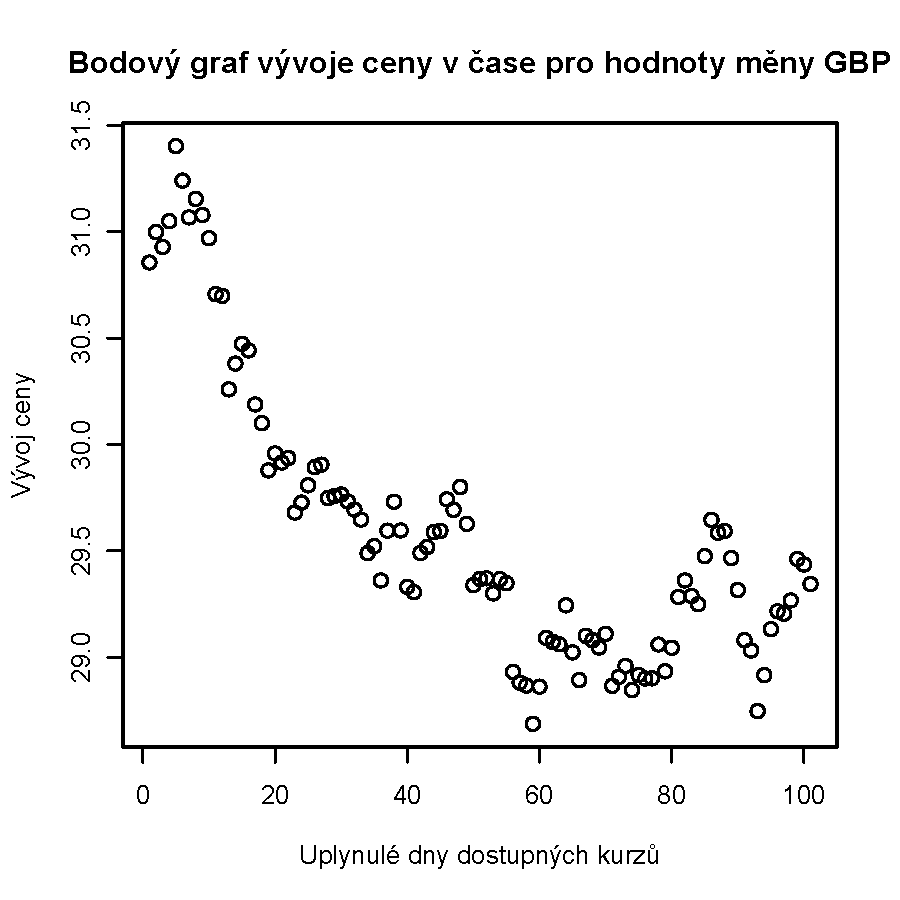
\includegraphics[width=10cm]{bodovy_max.pdf}
\caption{Bodový graf měny s maximální hodnotou šikmosti}
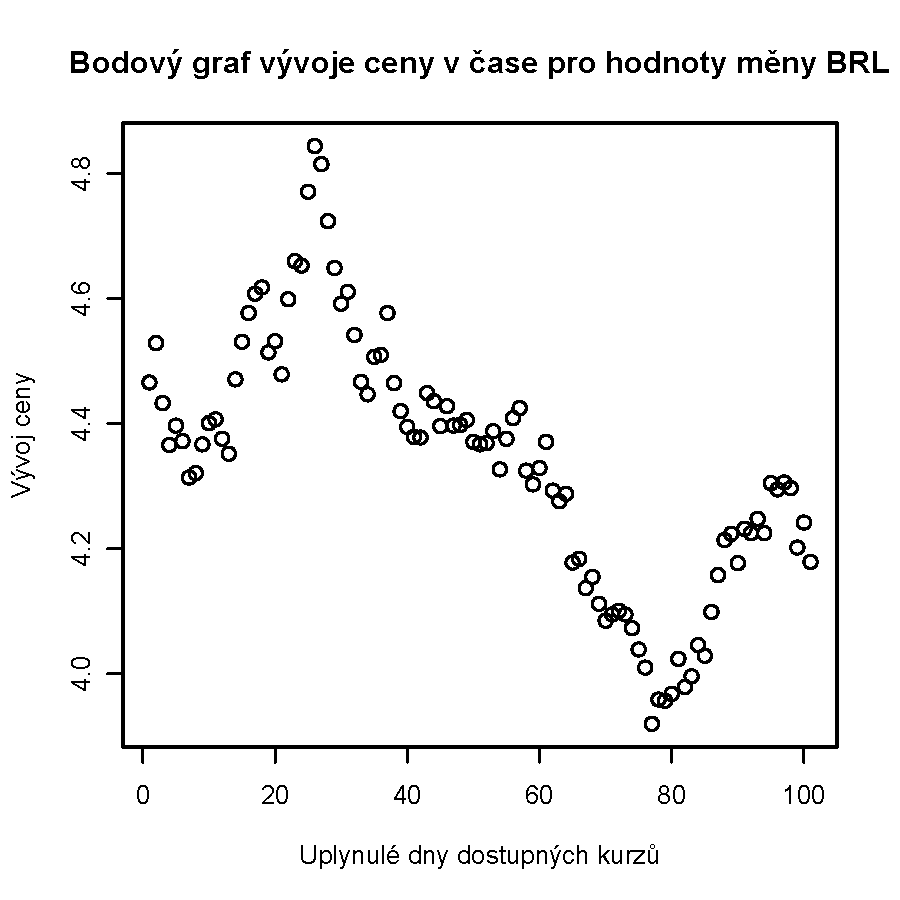
\includegraphics[width=10cm]{bodovy_min.pdf}
\caption{Bodový graf měny s minimální hodnotou šikmosti}
\end{figure}
\subsection{Hexbin}
\begin{figure}[H]
\centering
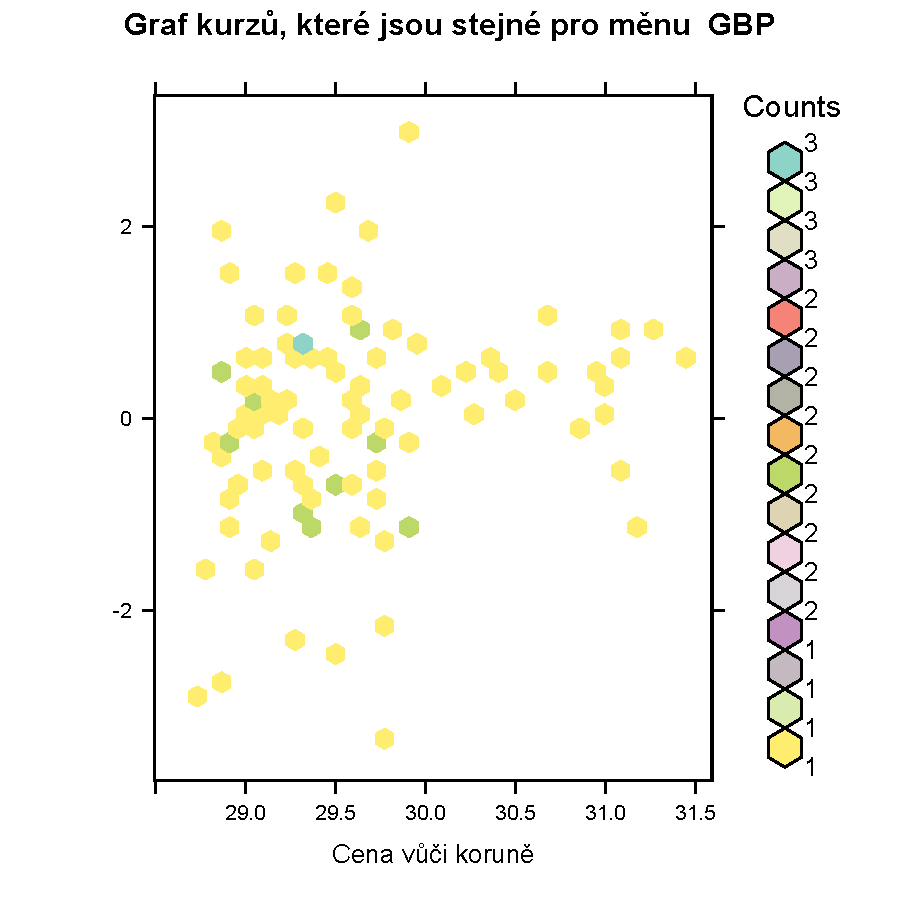
\includegraphics[width=10cm]{hexbin_graf_max.pdf}
\caption{Hexbin graf měny s maximální hodnotou šikmosti}
\centering
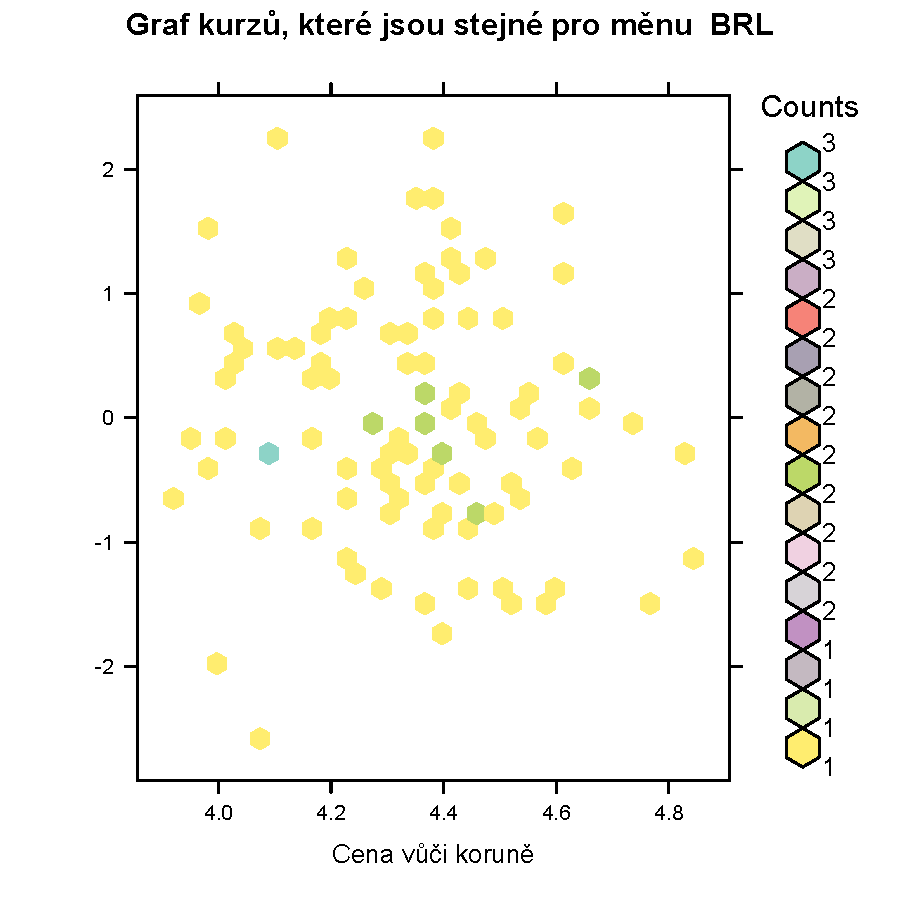
\includegraphics[width=10cm]{hexbin_graf_min.pdf}
\caption{Hexbin graf měny s minimální hodnotou šikmosti}
\end{figure}
\subsection{3D graf}
\begin{figure}[H]
\centering
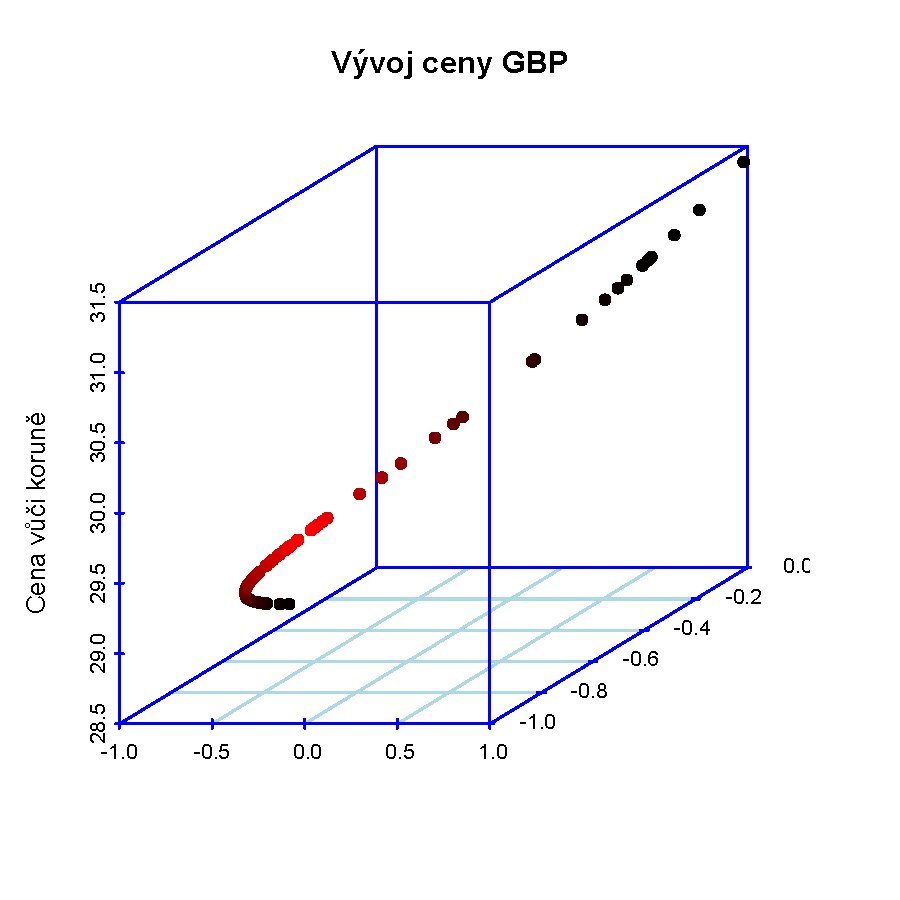
\includegraphics[width=10cm]{3D_graf_max.pdf}
\caption{3D graf graf měny s maximální hodnotou šikmosti}
\end{figure}
\begin{figure}[H]
\centering
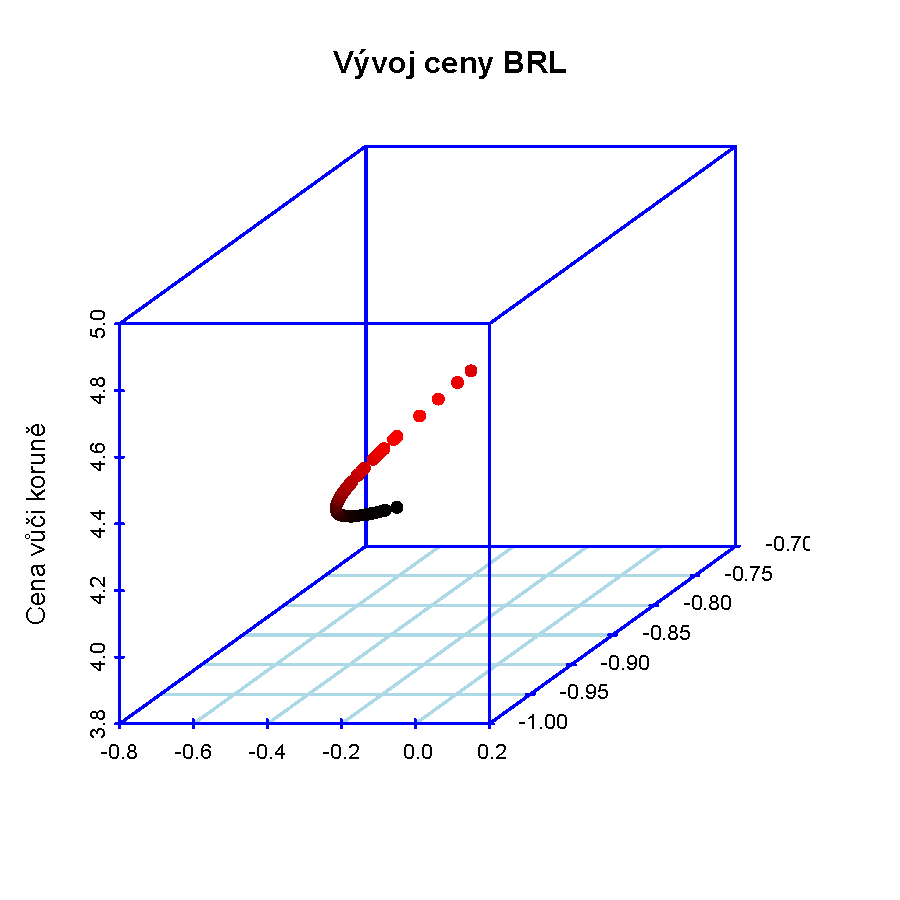
\includegraphics[width=10cm]{3D_graf_min.pdf}
\caption{3D graf graf měny s minimální hodnotou šikmosti}
\end{figure}
\subsection{Chernoff faces}
\begin{figure}[H]
\centering
\begin{Schunk}
\begin{Soutput}
effect of variables:
 modified item       Var  
 "height of face   " "USD"
 "width of face    " "GBP"
 "structure of face" "CHF"
 "height of mouth  " "EUR"
 "width of mouth   " "BRL"
 "smiling          " "ILS"
 "height of eyes   " "CAD"
 "width of eyes    " "MXN"
 "height of hair   " "BGN"
 "width of hair   "  "RON"
 "style of hair   "  "USD"
 "height of nose  "  "GBP"
 "width of nose   "  "CHF"
 "width of ear    "  "EUR"
 "height of ear   "  "BRL"
\end{Soutput}
\end{Schunk}
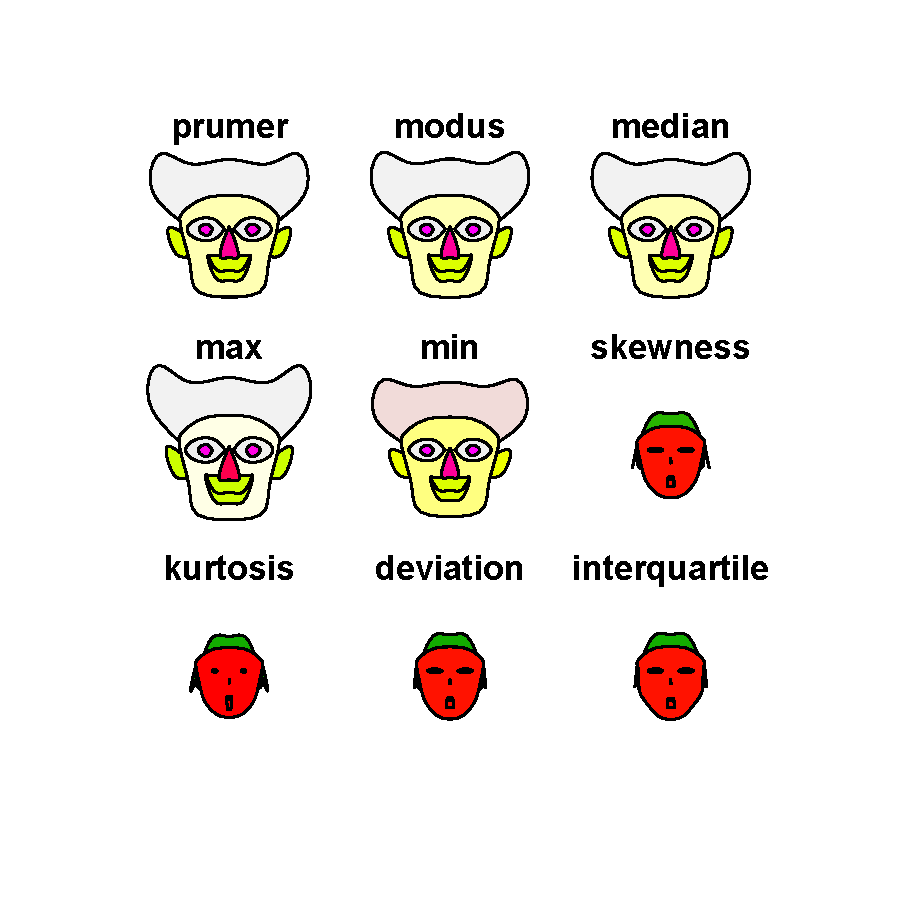
\includegraphics[width=10cm]{faces_graf.pdf}
\caption{Chernoff faces graf tabulky popisné statistiky}
\end{figure}
\clearpage

%% Testování statistických hypotéz
\section{Testování statistických hypotéz}
\subsection{Jednovýběrový Studentův test vůči střední hodnotě}
\begin{Schunk}
\begin{Soutput}
	One Sample t-test

data:  TestHypCur1
t = 31.433, df = 100, p-value < 2.2e-16
alternative hypothesis: true mean is not equal to 20
95 percent confidence interval:
 23.08508 23.50076
sample estimates:
mean of x 
 23.29292 
\end{Soutput}
\end{Schunk}
\subsection{Dvouvýběrový Studentův test}
\begin{Schunk}
\begin{Soutput}
	Welch Two Sample t-test

data:  TestHypCur1 and TestHypCur2
t = -51.224, df = 166.54, p-value < 2.2e-16
alternative hypothesis: true difference in means is not equal to 0
95 percent confidence interval:
 -6.549041 -6.062939
sample estimates:
mean of x mean of y 
 23.29292  29.59891 
\end{Soutput}
\end{Schunk}
\subsection{Fisherův test}
\begin{Schunk}
\begin{Soutput}
	F test to compare two variances

data:  TestHypCur1 and TestHypCur2
F = 2.6248, num df = 100, denom df = 100, p-value = 2.308e-06
alternative hypothesis: true ratio of variances is not equal to 1
95 percent confidence interval:
 1.769629 3.893242
sample estimates:
ratio of variances 
          2.624803 
\end{Soutput}
\end{Schunk}

%% ANOVA
\section{ANOVA}

%% Korelace
\section{Korelace}
\subsection{Korelační matice}
\begin{table}[H]
\begin{Schunk}
\begin{Soutput}
          USD       GBP       CHF       EUR       BRL       ILS       CAD
USD 1.0000000 0.9107230 0.9460180 0.9179658 0.6392782 0.9883873 0.9626825
GBP 0.9107230 1.0000000 0.8948676 0.8658716 0.4673841 0.9088316 0.8908392
CHF 0.9460180 0.8948676 1.0000000 0.9692083 0.4617732 0.9327882 0.9217226
EUR 0.9179658 0.8658716 0.9692083 1.0000000 0.5020093 0.9016465 0.9312468
BRL 0.6392782 0.4673841 0.4617732 0.5020093 1.0000000 0.6334782 0.6587888
ILS 0.9883873 0.9088316 0.9327882 0.9016465 0.6334782 1.0000000 0.9636070
CAD 0.9626825 0.8908392 0.9217226 0.9312468 0.6587888 0.9636070 1.0000000
MXN 0.6587680 0.5420454 0.5987799 0.7068223 0.7230531 0.6424965 0.7797695
BGN 0.9186576 0.8658093 0.9696949 0.9998681 0.5025878 0.9021541 0.9312349
RON 0.9480076 0.9012998 0.9807330 0.9928694 0.5247833 0.9318752 0.9408933
          MXN       BGN       RON
USD 0.6587680 0.9186576 0.9480076
GBP 0.5420454 0.8658093 0.9012998
CHF 0.5987799 0.9696949 0.9807330
EUR 0.7068223 0.9998681 0.9928694
BRL 0.7230531 0.5025878 0.5247833
ILS 0.6424965 0.9021541 0.9318752
CAD 0.7797695 0.9312349 0.9408933
MXN 1.0000000 0.7060044 0.6736579
BGN 0.7060044 1.0000000 0.9931094
RON 0.6736579 0.9931094 1.0000000
\end{Soutput}
\end{Schunk}
\caption{Korelační matice}
\end{table}
\subsection{Bodové grafy hodnot z korelační matice}
\begin{figure}[H]
\centering
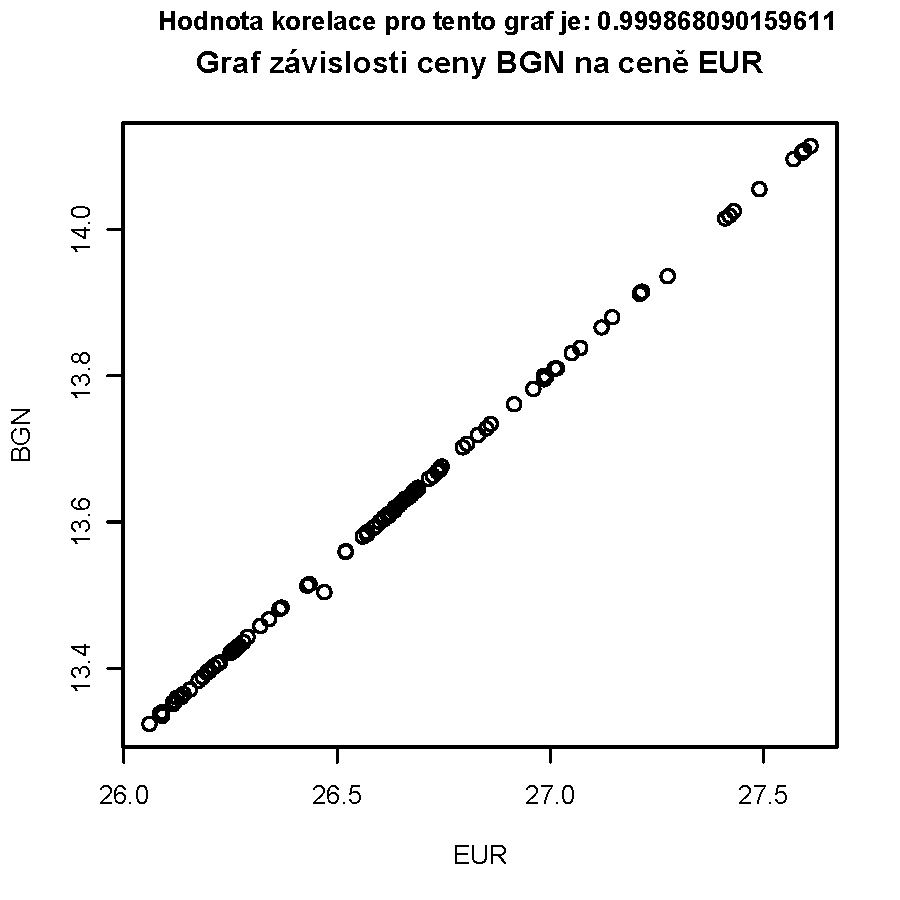
\includegraphics[width=10cm]{cor_max.pdf}
\caption{Bodový graf maximální hodnoty v korelační matici}
\end{figure}
\begin{figure}[H]
\centering
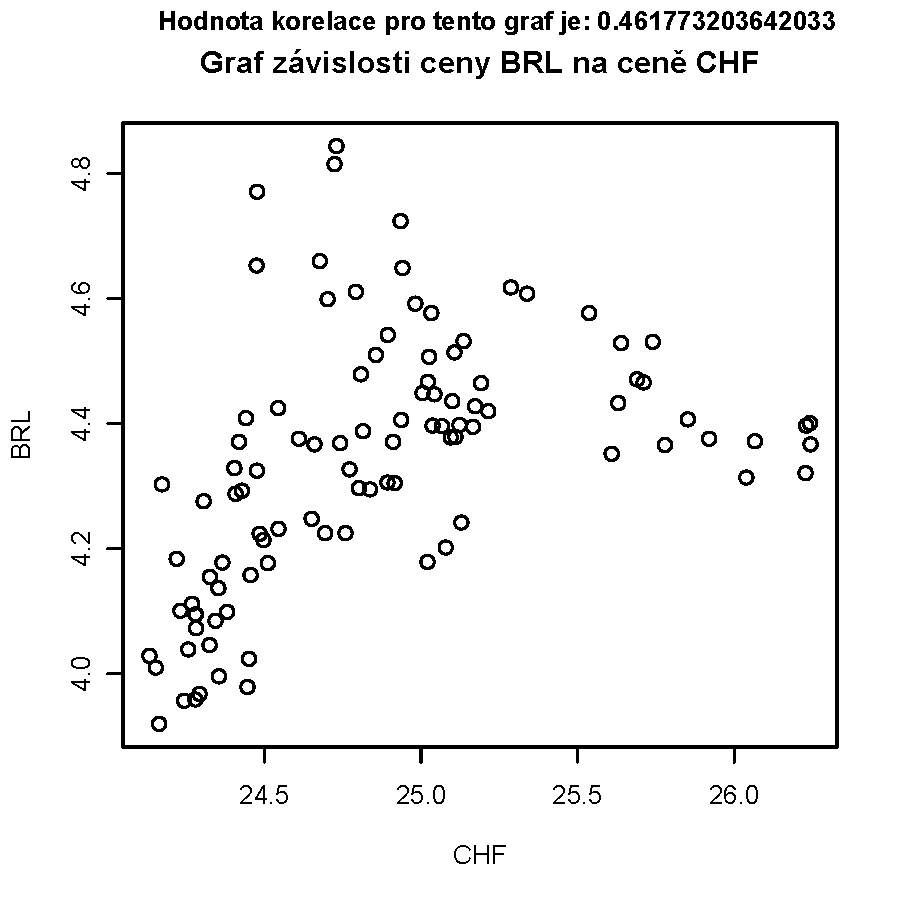
\includegraphics[width=10cm]{cor_min.pdf}
\caption{Bodový graf minimální hodnoty v korelační matici}
\end{figure}
\clearpage

%% Testování v kontingenčních tabulkách
\section{Testování v kontingenčních tabulkách}
\subsection{Chí kvadrát test}
\begin{Schunk}
\begin{Soutput}
	Chi-squared test for given probabilities

data:  smoke.freq
X-squared = 24.076, df = 3, p-value = 2.408e-05
\end{Soutput}
\begin{Soutput}
	Pearson's Chi-squared test

data:  kontTab
X-squared = 13.062, df = 6, p-value = 0.04206
\end{Soutput}
\begin{Soutput}
	Pearson's Chi-squared test

data:  kontTabSpojena
X-squared = 9.7686, df = 3, p-value = 0.02064
\end{Soutput}
\end{Schunk}
\section{Lineární regrese}
\begin{Schunk}
\begin{Soutput}
Call:
lm(formula = DATALregrese$lRegreseCur2 ~ DATALregrese$lRegreseCur1)

Coefficients:
              (Intercept)  DATALregrese$lRegreseCur1  
                 0.007772                   0.510974  
\end{Soutput}
\begin{Soutput}
Call:
lm(formula = DATALregrese$lRegreseCur2 ~ DATALregrese$lRegreseCur1)

Residuals:
       Min         1Q     Median         3Q        Max 
-0.0292594 -0.0001743  0.0003621  0.0011365  0.0035889 

Coefficients:
                           Estimate Std. Error t value Pr(>|t|)    
(Intercept)               0.0077722  0.0222232    0.35    0.727    
DATALregrese$lRegreseCur1 0.5109742  0.0008342  612.52   <2e-16 ***
---
Signif. codes:  0 '***' 0.001 '**' 0.01 '*' 0.05 '.' 0.1 ' ' 1

Residual standard error: 0.003296 on 99 degrees of freedom
Multiple R-squared:  0.9997,	Adjusted R-squared:  0.9997 
F-statistic: 3.752e+05 on 1 and 99 DF,  p-value: < 2.2e-16
\end{Soutput}
\end{Schunk}
\begin{figure}[H]
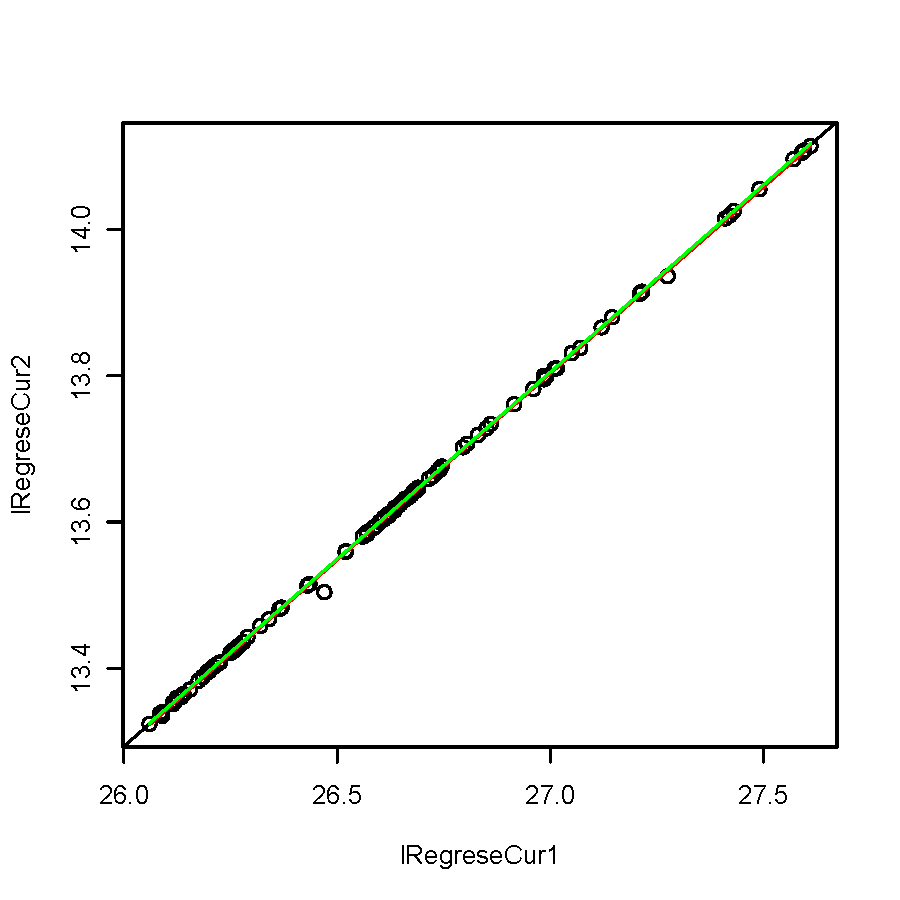
\includegraphics[width=10cm]{lregresePlot.pdf}
\caption{Graf lineární regrese}
\end{figure}
\clearpage

%%%%%%%%%%%%%%%%%%%%%%%%%%%%%%%%%%%%%%%%%%%%%%%%%%%%%%%%%%%%
% Závěr
%%%%%%%%%%%%%%%%%%%%%%%%%%%%%%%%%%%%%%%%%%%%%%%%%%%%%%%%%%%%

\clearpage \phantomsection \addcontentsline{toc}{section}{Závěr}
\section*{Závěr}

%%%%%%%%%%%%%%%%%%%%%%%%%%%%%%%%%%%%%%%%%%%%%%%%%%%%%%%%%%%%
% Použitá literatura
%%%%%%%%%%%%%%%%%%%%%%%%%%%%%%%%%%%%%%%%%%%%%%%%%%%%%%%%%%%%

\clearpage \phantomsection \addcontentsline{toc}{section}{\refname}

\begin{thebibliography}{99}	% parametr určuje nejširší položku

% nezlomitelné spojovníky lze zapisovat zkratkou "- nebo příkazem \babelhyphen{nobreak}

\bibitem{1}
Our World in Data
\textit{Data on COVID-19 (coronavirus)} [online]. 2021 [cit. 2021-11-18]. Dostupné z:~\url{https://github.com/owid/covid-19-data/tree/master/public/data}

\end{thebibliography}

%%%%%%%%%%%%%%%%%%%%%%%%%%%%%%%%%%%%%%%%%%%%%%%%%%%%%%%%%%%%
% Přílohy
%%%%%%%%%%%%%%%%%%%%%%%%%%%%%%%%%%%%%%%%%%%%%%%%%%%%%%%%%%%%

\clearpage \phantomsection \addcontentsline{toc}{section}{Seznam příloh}
\section*{Seznam příloh}

\noindent Příloha~A \dotfill \pageref{1}

% PŘÍLOHA A

\clearpage \phantomsection\label{prilohaA} \addcontentsline{toc}{section}{Příloha~A}
\section*{Příloha~A}

Příloha A zahrnuje ZIP soubor, který obsahuje: 

%%%%%%%%%%%%%%%%%%%%%%%%%%%%%%%%%%%%%%%%%%%%%%%%%%%%%%%%%%%%
% Konec dokumentu
%%%%%%%%%%%%%%%%%%%%%%%%%%%%%%%%%%%%%%%%%%%%%%%%%%%%%%%%%%%%

\end{document}

% vim:sw=8:ts=8
% EOF
